\documentclass[a4paper]{article}

\usepackage[english]{babel}
\usepackage[bitstream-charter]{mathdesign}
\usepackage[T1]{fontenc}
\usepackage[scaled]{beramono}
\usepackage{graphicx}
\usepackage{hyperref}
\usepackage{parskip}
\usepackage{listings}
\usepackage[usenames,dvipsnames]{xcolor}
\definecolor{dkgreen}{rgb}{0,0.6,0}

\lstset{
  aboveskip=3mm,%
  basewidth={0.58em, 0.53em},%
  basicstyle=\renewcommand{\baselinestretch}{0.95}\ttfamily,%
  belowskip=3mm,%
  breakatwhitespace=true,%
  breaklines=true,%
  captionpos=b,%
  columns=[c]fixed,%
  commentstyle=\itshape\color{dkgreen},%
  escapechar=¤,%
  firstnumber=0,%
  fontadjust=true,%
  framerule=0.3pt,%
  keepspaces=true,%
  frame=single,%
  keywordstyle=\bfseries\color{RoyalBlue},%
  language=Scala,%
  mathescape=true,%
  numbers=none,%
  numbersep=1.5mm,%
  numberstyle=\color{Magenta},%
  showstringspaces=false,%
  stringstyle=\color{Thistle},
  tabsize=2,%
  xleftmargin=4mm%
}
\newcommand{\code}[1]{%
    \lstinline[%keywordstyle=,%
               flexiblecolumns=true,%
               basicstyle=\ttfamily]#1}

% Put code in \cc{THE_CODE}, \cc{...} is shorter than \texttt{...}
\newcommand{\cc}[1]{\texttt{#1}}
% Put Scala code in \sc{THE_CODE}, the code will be syntax highlighted
% Use \cc{..} for class names
\renewcommand{\sc}[1]{\lstinline{#1}}
\newcommand{\field}[1]{\emph{#1}}
\begin{document}
\selectlanguage{english}

\title{Comparative Programming Languages\\
Assignment $^{\#}$2: Domain Specific Language}
\author{Glenn Croes \and Philippe De Croock \and Thomas Winant}
\date{11 January, 2012}

\maketitle

\tableofcontents

\section{Domain description}
\label{sec:domain-description}

% An elaboration on elements of the domain that were missing or needed to be improved, plus justification for any choices made.


% Vluchtnummer per vlucht, onafhankelijk van het vliegtuig
% Schedule-schedulItem kan mss nog worden verbeterd
% tijdstip per flight
% elke 1..* ipv 0..* in ons systeem
% Each flight of a certain flight template happens with the same airplane model

This section will reflect on the most important aspects of the problem domain.
We will not discuss the entirety of the problem domain or everything described in the assignment.
Only the important/changed parts are highlighted.

\begin{itemize}

\item It is necessary to support flexible modeling of flight schedules AND pricing (exceptions for holidays, variations in pricing etc.).
It must be possible to express statements such as ``The flight occurs every Wednesday and Friday at 16:30 except in July and August'' and ``In December and January the prices are increased by 20\%''.
We do assume flights have a recurring period of just one week (every Wednesday, every Monday,\dots).
The question if longer types of recurring schedules had to be supported (every two weeks, monthly,\dots) was posed to the domain expert, but no answer was given.
The assignment only describes weekly schedules:

\begin{quote}
Each code denotes a flight that recurs at the same time one or more days per week.
(Some flight takes place on just one day per week, others a couple of days per week, others every day.)
\end{quote}

So, for simplicity,  we decided to stick with just weekly recurring schedules.
Note: it is still possible to express variations and exceptions (e.g.\ every Wednesday except in January or every Monday except on December 25th)! \\

\item Each seat is assigned to a price category (\field{SeatType}).
Seats are priced individually, but prices fall into one of these categories.
Price categories are determined in advance.
However, a seat may change price category during a certain period (e.g.\ during high season).

\item The same flight can be serviced by multiple airplanes (even different airplane models).
We decided to treat \field{Airplane}s, \field{AirplaneModel}s and airplane \field{Manufacturer}s as separate entities.\\

\item Code-sharing flights (multiple companies for one flight) can be ignored as stated by the domain expert.\\

\item As hinted in the assignment, we decided to introduce the concept of a \field{FlightTemplate}.
A \field{FlightTemplate} describes a set of \field{Flight}s on the same \field{Connection}, serviced by a certain \field{AirlineCompany} with a certain schedule.
The flight's code is also determined by the \field{FlightTemplate}.
For example: all flights between Amsterdam and New York serviced by KLM. This \field{FlightTemplate} has the code KLM4753.
The flights occur every Wednesday at 14:00, except from the 20th of December until the 5th of January.


\item Flight details are available one year in advance. It is not necessary to generate flight data for an unlimited period of time (as stated by the domain expert).\\

\item Only the insertion of data into the database needs to be supported by the DSL.
Booking of flights and querying data is not part of our problem domain.
We also assume every entity is described in the DSL file.
No pre-existing entities are referred to.
For example: it is not possible to refer to a country ``Belgium'' if that country is not declared in the DSL file (but exists in the database).
We will not check everything that is already in the database before interpreting the DSL file.\\

\item The assignment states it should be possible to provide flight duration estimates.
We decided not to explicitly describe flight durations in \field{Flight}, but to keep track of the airplane's average cruise speed in order to be able derive the flight duration.
We assume the cruising speed is the most prominent factor that determines flight duration.
This should provide a better estimate of the flight's duration, as a flight may be serviced by different airplane models.\\


\end{itemize}

\section{Domain analysis}
\label{sec:domain-analysis}
% A brief breakdown of the elements in your domain and how they relate to each other. This could be a formal meta-model, but could also be textual description.

\begin{figure}[ht!]
  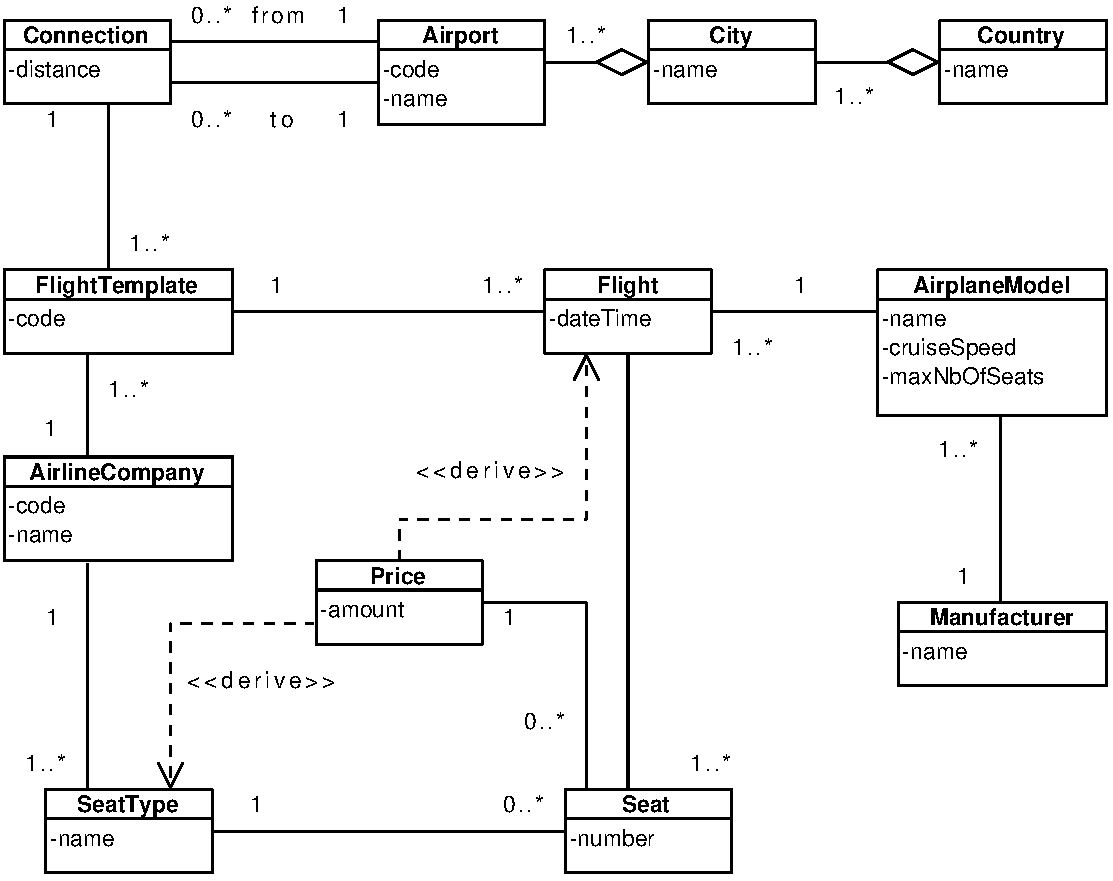
\includegraphics[width=1.0\textwidth]{../analysis/domainModel.pdf}
  \caption{Domain Model}\label{fig:domain-model}
\end{figure}

\paragraph{Country}
A \field{Country} has a name and represents a sovereign nation.
\paragraph{City}
A \field{City} has a name and is located in a \field{Country}.
\paragraph{Airport}
An \field{Airport} is located in a \field{City}.
It has a name and is uniquely identified by its 3 capital letter code.
It is possible for a city to have multiple airports.
\paragraph{Connection}
A \field{Connection} represents a flight link between two airports.
The distance in kilometers of the connection is stored.
A connection must be between two different airports.
\paragraph{AirlineCompany}
An \field{AirlineCompany} provides air transport services for passengers.
It has a name and is uniquely identified by a 2 or 3 capital letter code.
\paragraph{Manufacturer}
A \field{Manufacturer} is a business engaged in manufacturing airplanes.
Only the name of the manufacturer is relevant in our domain.
\paragraph{AirplaneModel}
An \field{AirplaneModel} is manufactured by a manufacturer.
It has a name and cruise speed.
The maximum number of seats that can be installed in the airplane model is stored too.
\paragraph{FlightTemplate}\label{par: flighttemplate}
A \field{FlightTemplate} describes a set of \field{Flight}s on the same \field{Connection}, serviced by a certain \field{AirlineCompany} with a certain schedule.
Each \field{FlightTemplate} is denoted by a unique code.
The code consists of the airline company's code followed by 3 to 4 digits.
An example: The \field{FlightTemplate} describing all flights between Amsterdam and Sydney serviced by KLM. This \field{FlightTemplate} has the code KLM4119.
The flights occur every wednesday at 12:00PM, except from the 20th of December until the 5th of January.

% TODO
% recurs at the same time one or more
% days per week
% flight that recurs at the same time one or more
% days per week. (Some flight takes place on just one day per week, others a
% couple of days per week, others every day.)
% To specify a specific flight, the date is also required.

% It is probably a good idea to separate the information about the flight and the
% ‘template’ describing flights. The ‘template’ includes the flight code, but the
% actual flight details include the date.

\paragraph{Flight}
A \field{Flight} is an instantiation of a flight template at a particular date and time.
As they are dependent on a flight template, flights are specific to airline companies.
A flight will happen with a certain airplane model.
\paragraph{SeatType}
A \field{SeatType} is used to define seat classes, for instance business and economy are two seat types.
Only the name of the seat type is stored.
Different airline companies can reuse the same seat types.
\paragraph{Seat}
A \field{Seat} represents a seat on a flight.
A seat has a seat number that is unique on the airplane.
\paragraph{Price}
Every seat on a flight has a \field{Price}.
The price depends on the flight and the seat type.
This means that two seats, both of the same seat type and both on flights that follow the same template, can have different prices on different dates.



\begin{figure}[ht!]
  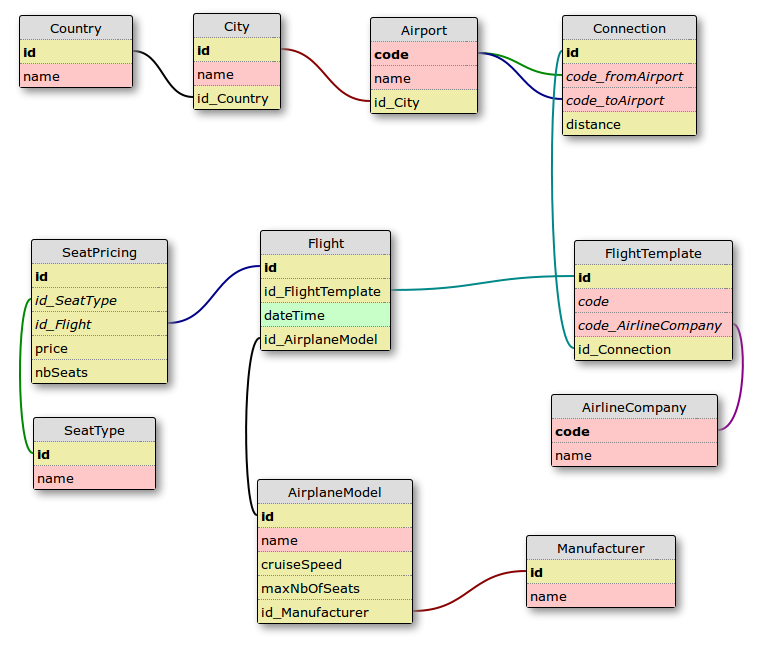
\includegraphics[width=1.0\textwidth]{../analysis/dbtables-diagram.png}
  \caption{Database Tables}\label{fig:database-tables}
\end{figure}

\section{Design Description}
\label{sec:design-description}

% A description of the semantic model underlying the DSL, along with a description of the constructs of your DSL.

% A general overview of the implementation approach, including a description of the API upon which it is based and any tricky implementation techniques employed. Some justification of the chosen implementation language needs also to be provided.

%% TODO Fix the text below

Before a high-level walk through the implementation, we shall first describe the design behind our DSL.
The idea is to define Cities, Airports, Flights, \ldots{} using an easy to use and intuitive syntax.
All defined \emph{entities} will then be stored in a database.
Flight entities are generated from FlightTemplates using a \cc{Schedule} and a \cc{Pricing\-Scheme} (more about these later).
The database is populated after all entities are defined and the required consistency checks are performed.
Communication with the database happens through \textsc{JDBC} (Java Database Connectivity).
As we're using \textsc{JDBC}, we could support a whole host of different database types.
Currently, we support SQLite (no extra setup required, as the database is stored in a file), which is also the default, and MySQL (one of the most popular database products).
After running our DSL program, the database will contain the rows defined using the DSL.\@

We first intended to generate SQL scripts that would insert the generated entities in the database when executed, but this proved to be difficult because of the following reason.
Imagine we want to generate an \cc{INSERT} statement that would insert a new City in the database.
A City consists of a name of type String, and a country of type Country, which is another entity (or table).
In the database table, the country field of the City table is defined as a foreign key that references the Country table via Country's primary key (an auto-generated ID).
How would such an \cc{INSERT} statement then look like?

\cc{INSERT INTO City (name, id\_Country) VALUES ("Brussels", ?)}

Which value should come in the place of the question mark?

The right thing to do, would be to insert the value of the auto-generated ID of the row representing Belgium in the Country table, but we don't know the value of this ID, as we haven't inserted Belgium it in the database yet.
A possible alternative is to switch to manually generated IDs, but extra attention would have to be paid to prevent conflicts with existing IDs.
We believe directly communicating with the database at run-time and retrieving the IDs after they were generated, is a more robust solution.


\section{Implementation Overview}
\label{sec:implementation-overview}

% A general overview of the implementation approach, including a description of the API upon which it is based and any tricky implementation techniques employed. Some justification of the chosen implementation language needs also to be provided.

To implement the database functionality, we use the JDBC API. 
The reason for this is because SQL scripts seem difficult to do, as discussed later on. %TODO link?
Also, the use of such an API is safer and more coherent.

No loose strings have been used to insert sql statements into the database.
All SQL statements have to be prepared using the PreparedStatements class.
Using loose strings to insert statement could introduce errors or make it possible to hack the database by, for example, SQL injection.

To create such a PreparedStatement, a prepareStatement function has been written.
The method expects a connection to the specific database, an SQLDataTypeMapper and an IDMap.
The statement will be constructed like this:
\begin{verbatim}
val prepStr = "INSERT INTO %s (%s) VALUES (%s)"
\end{verbatim}
This string will then be formatted to fill in the placeholders with the right arguments.
The SQLDataTypeMapper makes sure the defined types of Scala and the types of the SQL database are compatible.
Afterwards, the string is prepared and executed using the prepareStatement method of Connection.
\subsection{Implementation language}
\label{sec:implementation-language}

We chose to implement our DSL in Scala for the following reasons:

\paragraph{Static Typing}
Scala is statically typed and has a rather advanced type system.
Scala's type system allows us to express and verify more complex types of expressions.
A whole class of consistency checks related to types can be eliminated in the DSL, thanks to static typing.

\paragraph{Familiarity}
Although only one group member had experience with programming in Scala before the \textsc{CPL} course, Scala is not too unfamiliar for experienced Java programmers.
Syntactically, Scala is quite similar to Java.
Programmers familiar with the object-oriented paradigm as it is applied in Java, can start programming in Scala relatively easy, as the \textsc{OO} paradigm is also present in Scala, albeit enhanced and combined with the functional programming paradigm.

\paragraph{Feature Set}
Scala provides programmers with many useful building blocks for developing DSLs, including, but not limited to:

\begin{itemize}
\item \textbf{Implicits arguments and conversions}:
  Implicit arguments alleviate the need to pass around certain parameters, making the program less verbose and more intuitive to read (at times).
  Implicit conversions provide an easy way to add functionality to existing classes, we used it mainly to add syntactic sugar (see Section~\ref{sec:implementation-syntax}).
\item \textbf{Operator syntax}:
  Scala supports the definition of operators just like methods, e.g.\ \sc{BRU -> CDG} is actually a method call.
  The dot and parentheses in a functional call can be omitted in certain circumstances, allowing more natural language-like syntax, e.g.\ \sc{"Brussels" in Belgium}.
\item \textbf{Traits}:
  Traits are (also) a useful way to structure to code into units of functionality.
  Instead of being forced to stick to a strict inheritance relation, or to put all code in one place, we can compartmentalize the functionality into different traits.
\end{itemize}

\paragraph{Scala 2.9 vs 2.10}

We used Scala version 2.9.2 to implement our DSL.
Although version 2.10, which includes many useful enhancements, was recently released, it (or at least a final version) wasn't available at the start of the assignment.
Scala 2.10 has (experimental) support for macros, a very powerful and much wished-for tool for DSL designers.
Implicit classes are also available in 2.10, which reduce the boilerplate required for some of the tricks described in Section~\ref{sec:implementation-syntax}.
Another useful addition is the \cc{Dynamic} type: ``\sc{x.foo} becomes \sc{x.applyDynamic("foo")} if \sc{x}'s type does not define a \sc{foo}, but is a subtype of \cc{Dynamic}''.
This trick, the equivalent of Ruby's \cc{method\_missing}, would be very useful to support extra syntax.
In hindsight, our DSL could have been much \emph{prettier} if we used Scala 2.10, but because the final version was released only recently (January 4th) and because of time constraints, we chose to stick to the latest stable release, 2.9.2.


\subsection{General Implementation Overview}
\label{sec:general-implementation-overview}

Now follows a high-level tour of the most important parts of our DSL implementation.
The name of the source file is mentioned in bold.
More details can be learned from reading the source files, which are provided with commentary.

\paragraph{DBDefinition.scala}
First of all, we defined case classes for every table or \cc{Entity} in the database.
The fields of a table correspond with the fields of the case classes, except for the auto-generated keys.
Custom fields, like \cc{Airport\-Code} and \cc{Air\-line\-Code}, were defined as well.

\paragraph{DBDSL.scala}
We used a tiny DSL to define these entities (tables).
This DSL contains the \cc{Entity} trait, that all tables extend.
An Entity can insert itself into a database using a \cc{PreparedStatement}.

\paragraph{DateAndTime.scala}
We defined a number of auxiliary classes (\cc{WeekDay}, \cc{Month}, \cc{Date}, \cc{Time}, and \cc{DateTime}) for working with dates and times.
These classes are mostly wrappers for existing classes from the \href{http://joda-time.sourceforge.net/}{Joda-time library} that provide extra syntactic sugar and methods.
We chose not to implement the extra functionality in the form of implicit conversions, as the users of our DSL are already working with custom syntax and don't come in touch with the underlying types.

\paragraph{SQLPopulator.scala}
To support multiple types of databases (currently SQLite and MySQL), we abstracted the common functionality of databases in a trait, \cc{SQL\-Populator}.
Adding support for a new type of database requires the definition of a new trait that implements the abstract members of SQLPopulator.
The only abstract member of this trait is:

\sc{def connect(jdbcString: String): Connection}

This method will be called only once, should load the correct JDBC driver, and return a new connection to the database.
Also present is the \cc{SQLDataTypeMapper} trait, which takes care of filling in a PreparedStatement with the appropriate methods, e.g.\ \cc{Prepared\-State\-ment\-\#set\-String(..)}, \cc{Prepared\-State\-ment\-\#set\-Int(..)}, etc.
The default methods in this trait can also be overriden by database-specific ones, as for example SQLite does not support the \cc{Prepared\-State\-ment\-\#set\-Big\-Decimal(..)} method.
The user of our DSL can choose which database to use by mixing-in the database-specific SQLPopulator trait (\cc{SQLitePopulator} or \cc{MySQL\-Populator}) of his choice.

\paragraph{FlightDSL.scala}
The actual DSL that will be used by users is defined in \cc{Flight\-DSL.scala}.
The DSL provides lot of syntactic sugar for defining the Countries, Cities, Airports, Manufacturers (of airplanes), Airplane Models, Airline Companies, Seat Types, and Flight Templates.
All entities of a certain type defined by the user using DSL syntax are also stored in a Vector.
At the end, all Vectors are stored in the database.

In our DSL, the user defines Flight Templates from which Flights are generated.
A Flight is an instantiation of a Flight Template at a certain date and time.
To generate Flights at certain points in time, a Schedule is used.
A Schedule is defined through composition.
Have a look at the following example:
\begin{lstlisting}
val wholeYear = (1 January 2013) -> (31 December 2013)
new Schedule()
 .at(9 h 55, every(Monday) during wholeYear) {
  Business -> (25.seats at 250.EUR);
  Economy -> (110.seats at 150.EUR)
}.except(6 January 2013, 25 December 2013)
 .at(15 h 3, 24 December 2012) {
  Business -> (20.seats at 400.EUR);
  Economy -> (125.seats at 300.EUR)
}
\end{lstlisting}

The first line in the example defines an interval between the beginning of 2013 and the end of 2013, i.e.\ the year 2013.
The Schedule that is defined states that every Monday of the year, a flight at five to ten in the morning with 25 business seats for 250 euros and 110 economy seats for 150 euros is planned, except on Christmas (if Christmas happened to fall on a Monday in 2013).
An additional flight is added that flies on the 24th of December, but with higher prices.

A Schedule object stores a sequence of moments when flights would occur, along with pricing information per seat class.
Flight objects will be generated for every moment in the Schedule.

To give maximum control over pricing information, we also introduced Pricing Schemes, which are Airline Company-specific.
A Pricing Scheme consists of a partial function from Seat Type, Date, and Price to Price.
It provides users an easy way to adjust prices on flights on certain dates and per Seat Type.
Have a look at the following example:

\begin{lstlisting}
new PricingScheme {
  def inSummer(date: Date): Boolean =
    date.in(21 June 2013, 21 September 2013)

  val highSeason: PricingScheme = {
    case (_, date, price) if inSummer(date) => price * 1.1
  }

  val firstClassTax: PricingScheme = {
    case (FirstClass, _, price) if price > 500.EUR
      => price + 50.EUR
  }

  val scheme = highSeason andAlso firstClassTax
}
\end{lstlisting}

A helper method is defined, \sc{inSummer}.
Two partial functions are defined and composed to form the \sc{scheme}, the abstract partial function member that must be implemented.
The first partial function, \sc{highSeason}, raises the price of flights in the summer by 10\%.
The second partial function, \sc{firstClassTax}, raises the price of first class flights by 50 euros if the price of the flight exceeds 500 euros.

We believe Pricing Schemes give users enough control over flight pricing.
Of course, additional input parameters could be added, like the Airplane Model or the time of departure, but such changes require only little work.
Users that wish not to use Pricing Schemes can provide a simple fall-through Pricing Scheme that doesn't influence the price at all.

\subsection{Consistency checks}
\label{sec:consistency-checks}
The following consistency checks are made before data is stored in the database:

\begin{itemize}
 \item Date and Time must be valid (0<hours<24, 0<minutes<60, \dots). Some of these checks are done by the Joda-Time library.
 \item The number of seats that gets assigned a price cannot exceed the number of seats on the flight (the number of seats on the airplane model servicing the flight).
 \item The code of a flight must be unique.
 \item A flight template must generate at least one flight.
 \item An airport code must consist of 3 capital letters.
 \item An airline company code must consist of 2 to 3 capital letters.
 \item A flight number must consist of 3 to 4 digits.
 \item The departure and arrival airports of a connection must be different (you cannot fly to the same airport).
 \item The total number of seats on a flight must be at least one.
 \item There must be at least one seat type on a flight.
 \item The number of seats assigned to a seat type must be at least one.
 \item The price of a seat cannot be negative.
 \item The number of passengers an airplane can carry cannot be negative.
 \item The cruise speed of an airplane must be larger than zero km/h.
\end{itemize}

The static typing of Scala provides consistency of types.

\subsection{Implementations Techniques}
\label{sec:implementation-techniques}

A pattern (or trick) we often used to add some syntactic sugar is the following.
Suppose we want to define a city, Brussels for instance, in our DSL.\@
\cc{City} is a case class with the following definition:

\sc{case class City(name: String, country: Country)}\ldots{}

Instead of \sc{val Brussels = City("Brussels", Belgium)} (\cc{Belgium} is an existing value of type \cc{Country}), we would like to define the city in a style resembling natural language.\\
For example: \sc{val Brussels = "Brussels" in Belgium}.\footnote{It's a shame we have to mention ``Brussels'' twice.}
The \sc{in} in the example above is actually a method call on the string \cc{Brussels} with \cc{Belgium} as sole argument.
Of course, there is no \sc{in} method taking a \cc{Country} defined for strings.
Using implicit conversions we can easily implement it:

\begin{lstlisting}
implicit def cityIn(cityName: String) = new {
  def in(country: Country) = City(cityName, country)
}
\end{lstlisting}

The code above defines an implicit conversion from a string (\sc{cityName}) to a new object on which the method \sc{in(country: Country)} is defined which returns a newly constructed \cc{City} object.

We also applied this pattern to provide a pretty syntax to define dates, e.g.\ \sc{val christmas = 25 December 2013}.
\cc{December} is actually a method defined on \cc{Int} (the day of the month) that takes a year argument.

This pattern can be applied recursively to form a sentence where method calls connect arguments together.\\
E.g.\ \sc{"Airbus A320" of Airbus carries 150.p flies 828.kmh}\\
The required implicit conversion:

\begin{lstlisting}
implicit def airplaneModelOf(modelName: String) =  new {
  def of(company: Manufacturer) = new {
    def carries(passengers: Passengers) = new {
      def flies(speed: Kmh): AirplaneModel =
        AirplaneModel(modelName, passengers.ps,
                      speed.kmhs, company)
    }
  }
}
\end{lstlisting}

As you can see in the example above, some numbers have a suffix to make their meaning clearer.
For example, the \sc{.kmh} in \sc{flies 828.kmh} immediately makes clear that the number is actually the speed, expressed in km/h.
Without the suffix, it could mean anything, e.g.\ ``flies 828 around the world before requiring maintenance''.
This is another trick we often applied to improve the legibility of our DSL.
The suffix is actually a method defined on \cc{Int} via an implicit conversion.
The implicit conversion that facilitates this:
\begin{lstlisting}
case class Kmh(kmhs: Int)

implicit def kmhUnit(kmhs: Int) = new {
  def kmh: Kmh = Kmh(kmhs)
}
\end{lstlisting}

By defining separate case classes for these unit types instead of relying on the built-in types like \cc{Int} or \cc{Double}, the type checker will signal a type error whenever a user of our DSL forgets a suffix that converts a number to the right unit type.
Of course, we could make it more extensible by defining a trait for speed, which \cc{KmH} and other classes like \cc{MpH} could implement, but this is a small change that could easily be made when necessary.


\section{DSL Implementation}
\label{sec:dsl-implementation}

% The code implementing your DSL and any libraries on which it is based.

\section{Example DSL program(s)}
\label{sec:example-dsl-programs}

% Some example DSL programs to illustrate how your DSL is to be used.

We shall now walk through an example DSL program in its entirety.
Code fragments will be interleaved with descriptive comments.
The complete example can also be found in the submitted source code.


We start with the definition of the \cc{Example} object.
To have access to the DSL functionality, it must extend the \cc{FlightDSL} trait.
Also, by mixing-in the SQLitePopulator trait, the user declares that he wishes to use an SQLite database.
Auxiliary methods are imported from the \cc{Date}, \cc{Month}, and \cc{WeekDay} objects.
Finally, a JDBC string that declares how the program should connnect to the database, called \cc{test.db}, is defined.

\begin{lstlisting}
package globair
object Example extends FlightDSL with SQLitePopulator {
  import Date._
  import Month._
  import WeekDay._

  val dbName = "jdbc:sqlite:test.db"
\end{lstlisting}

Next, Countries, Cities, Airports, Manufacturers, and Airplane Models are defined.
The Airport and Airplane Model values will be used later on in the example.

\begin{lstlisting}
// Countries
val Belgium = country("Belgium")
val France = country("France")
val Germany = country("Germany")
val Italy = country("Italy")
val Sweden = country("Sweden")

// Cities
val Brussels = "Brussels" in Belgium
val Paris = "Paris" in France
val Frankfurt = "Frankfurt" in Germany
val Rome = "Rome" in Italy
val Stockholm = "Stockholm" in Sweden

// Airports
val BRU = ("BRU", "Brussels Airport") at Brussels
val CDG = ("CDG", "Charles de Gaulle Airport") at Paris
val FRA = ("FRA", "Frankfurst am Main Airport") at Frankfurt
val CIA = ("CIA", "Rome Ciampino Airport") at Rome
val ARN = ("ARN", "Stockholm Arlanda Airport") at Stockholm

// Manufacturers
val Airbus = manufacturer("Airbus")
val Boeing = manufacturer("Boeing")

// Airplane Models
val AirbusA380 = "Airbus A380" of Airbus carries 644.p flies 945.kmh
val Boeing727 = "Boeing 727" of Boeing carries 145.p flies 963.kmh
val Boeing737_800 = "Boeing 737-800" of Boeing carries 160.p flies 828.kmh
\end{lstlisting}

Two divisions of Seat Types are then defined.
Some Airline Companies will have Business and Economy seats, others will divide the seats into three classes.
Multiple Airline Companies are allowed to share the same Seat Types.
Only two kinds of divisions were defined for the example, in \emph{reality}, more hierarchies would be defined, possibly with names specific to the Airline Company.

\begin{lstlisting}
// Two kinds of seats: Business and Economy
val Business = seatType("Business")
val Economy = seatType("Economy")

// Three kinds of seats: First, Second, and Third Class
val FirstClass = seatType("First Class")
val SecondClass = seatType("Second Class")
val ThirdClass = seatType("Third Class")
\end{lstlisting}

What follows is the definition of an Airline Company value for British Midlands.
The definition of an Airline Company includes the definition of its Pricing Scheme.
First, a local helper function is defined to determine whether a \cc{Date} lies in the high season, which is defined from the first day of July to the last day of August and from December 15th to March 31st the next year.
The Pricing Scheme consists of a single partial function, called \cc{highSeason}, which should be read as follows.
The price for Business seats is raised by 10\% in the high season.
The price for Economy seats is raised by 5\% in the high season.

\begin{lstlisting}
// Airline Companies (the code is the official IATA code)
val BM = company("BM", "British Midlands Airways",
                 new PricingScheme {

  def inHighSeason(date: Date): Boolean =
    date.in(1 July 2013, 31 August 2013) ||
    date.in(15 December 2013, 31 March 2014)

  val highSeason: PricingScheme = {
    case (Business, date, price) if inHighSeason(date)
      => price * 1.1
    case (Economy, date, price) if inHighSeason(date)
      => price * 1.05
  }

  val scheme = highSeason
})
\end{lstlisting}

Another Airline Company is defined, SN Brussels Airlines.
Its Pricing Scheme should be read as follows.
The price of flights in the summer is raised by 10\%.
There is also a special action on second class seats from July 15th to August 15th, during which a 50 euro discount applies.
SN Brussels Airlines also has another special action, called Back to School from August 16th to the end of August, during which a 10 euro discount on third class seats applies.
The \sc{scheme} definition at the end, states that first the \cc{highSeason} partial function is applied, then \cc{special\-Action\-On\-Second\-Class}, and finally \cc{backToSchool}.
Note that we use \sc{andAlso} to compose the partial functions, which applies both the first and the second partial function, even if the first didn't match, unlike \sc{andThen}.

\begin{lstlisting}
val SN = company("SN", "SN Brussels Airlines", new PricingScheme {

  def inSummer(date: Date): Boolean =
    date.in(21 June 2013, 21 September 2013)

  val highSeason: PricingScheme = {
    case (_, date, price) if inSummer(date) => price * 1.1
  }

  val specialActionOnSecondClass: PricingScheme = {
    case (SecondClass, date, price) if date.in(15 July 2013, 15 August 2013) => price - 50.EUR
  }

  val backToSchool: PricingScheme = {
    case (ThirdClass, date, price) if date.in(16 August 2013, 31 August 2013) => price - 10.EUR
  }

  val scheme = highSeason andAlso specialActionOnSecondClass andAlso backToSchool
})
\end{lstlisting}

Now follows the definition of a Flight Template for British Midlands.
First, some auxiliary values are defined, \sc{wholeYear} and \sc{summer}, each an interval between two days.
Also \sc{wholeWeek} is defined, a sequence of all the Week Days.
These will be used to define the Schedule of the Flight Template.

The Flight Template describes Flights with code number BM1628, flying between Brussels Airport (BRU) and Charles de Gaulle Airport (CDG).
The distance between the airports is 252 km.
The Flights will happen with a Boeing 727 airplane, every Monday of the year at 9:55, every Friday during the summmer at 10:09.
But not on January 6th and Christmas day (if they were a Monday or a Friday)
An additional Flight is scheduled on December 24th.
For every planned flight, the number of seats of each class and the price is also supplied (this information will be the same for all instances of the same recurring flight).

Another small Flight Template describes Flights between Frankfurt Airport and Stockholm Airport on every Saturday of the year.

\begin{lstlisting}
// Flights

val wholeYear = (1 January 2013) -> (31 December 2013)
val summer = (21 June 2013) -> (21 September 2013)

val wholeWeek = Monday -> Sunday

// British Midlands
FlightTemplate(BM, 1628)(BRU -> CDG, 252.km)(Boeing727) {
  new Schedule()
    .at(9 h 55, every(Monday) during wholeYear) {
    Business -> (25.seats at 250.EUR);
    Economy -> (110.seats at 150.EUR)
  }.at(10 h 9, every(Friday) during summer) {
    Business -> (30.seats at 300.EUR);
    Economy -> (115.seats at 200.EUR)
  }.except(6 January 2013, 25 December 2013)
    .at(15 h 3, 24 December 2013) {
    Business -> (20.seats at 400.EUR);
    Economy -> (125.seats at 300.EUR)
  }
}

FlightTemplate(BM, 2439)(FRA -> ARN, 1227.km)(Boeing737_800) {
  new Schedule()
    .at(4 h 23, every(Saturday) during wholeYear) {
    Business -> (40.seats at 350.EUR);
    Economy -> (120.seats at 250.EUR)
  }
}
\end{lstlisting}

Lastly, a Flight Template for SN Brussels Airports is defined between Brussels and Rome.
The Flights happen every day of the week during the summer.

\begin{lstlisting}
// SN Brussels Airlines
FlightTemplate(SN, 324)(BRU -> CIA, 1187.km)(AirbusA380) {
  new Schedule()
    .at(21 h 40, wholeWeek during summer) {
    FirstClass -> (42.seats at 600.EUR);
    SecondClass -> (102.seats at 325.EUR)
    ThirdClass -> (500.seats at 287.EUR)
  }
}

// End of the program
\end{lstlisting}

\section{DSL Cheat sheet}
\label{sec: cheat-sheet}

This section summarizes how to define each entity in the DSL.
Text between `$<$' and `$>$' symbols denotes variables.
Text between `$[$' and `$]$' denotes grouping of (optional) text.
A `$|$' symbolizes a logical or.
A `$^*$' denotes that an element can be repeated zero ore more times.
A `$^+$' denotes that an element can be repeated one ore more times.
example: $[a|b|c]^*$ denotes multiple $a$, $b$ or $c$'s ($aa$, $aabc$, \dots).

An example is given for every syntax element.

\newcommand{\elem}[1]{\vspace{-1.5em}\paragraph{#1}\hfill}

\elem{Date}
\begin{lstlisting}
<DD Month YYYY>

example:
val christmas = 25 December 2013
\end{lstlisting}

\elem{Date Ranges / intervals}
\begin{lstlisting}
(<fromDate>) -> (<toDate>)

example:
val wholeYear = (1 January 2013) -> (31 December 2013)
val summer = (21 June 2013) -> (21 September 2013)
\end{lstlisting}

\elem{Time}
\begin{lstlisting}
<hours> h <minutes>

example:
val noon = 12 h 00
\end{lstlisting}

\elem{Weekday}
\begin{lstlisting}
<Weekday>

example:
Monday
\end{lstlisting}

\elem{Weekday Range}
\begin{lstlisting}
<fromWeekday> -> <toWeekday>

example:
val wholeWeek = Monday -> Sunday
val longWeekend = Friday -> Monday
\end{lstlisting}
\clearpage

\elem{Weekly recurrences}
\begin{lstlisting}
every(<Weekday>+)

example:
every(Monday)
every(Monday, Wednesday, Friday)
\end{lstlisting}

\elem{Weekly recurrences during interval}
\begin{lstlisting}
every(<Weekday>+) during <interval>

example:
val summer = (21 June 2013) -> (21 September 2013)
every(Monday, Tuesday) during summer
\end{lstlisting}

\elem{Country}
\begin{lstlisting}
val <valName> = country("<countryName>")

example:
val Belgium = country("Belgium")
val Italy = country("Italy")
\end{lstlisting}

\elem{City}
\begin{lstlisting}
val <valName> = "<cityName>" in <country>

example:
val Brussels = "Brussels" in Belgium
val Rome = "Rome" in Italy
\end{lstlisting}

\elem{Airport}
\begin{lstlisting}
val <valName> = ("<airportCode>","<airportName>") at <city>

example:
val BRU = ("BRU", "Brussels Airport") at Brussels
val CIA = ("CIA", "Rome Ciampino Airport") at Rome
\end{lstlisting}

\elem{Manufacturer}
\begin{lstlisting}
val <valName> = manufacturer("<manufacturerName>")

example:
val Airbus = manufacturer("Airbus")
\end{lstlisting}
\clearpage

\elem{Airplane Model}
\begin{lstlisting}
val <valName> = "<modelName>" of <manufacturer> carries <nbOfSeats>.p flies <speedInKmph>.kmh

example:
val AirbusA320 = "Airbus A320" of Airbus carries 150.p flies 828.kmh
\end{lstlisting}

 \elem{Seat Type}
\begin{lstlisting}
val <valName> = seatType("<seatTypeName>")

example:
val Business = seatType("Business")
\end{lstlisting}

\elem{PricingScheme}
\begin{lstlisting}
new PricingScheme {
  [<optional helper methods>]
  [
  val <schemeName>: PricingMatcher = {
    [
    case (<seatType>, <date>, <price>) [if <condition>] =>
        <priceCalculation>
    ]*
  }
  ]*
  val scheme = <schemeName> [
          [AndAlso|OrElse|AndThen] <otherSchemeName>
        ]*
}

example:
new PricingScheme {
    def isHighSeason(date: Date): Boolean =
      date.in(15 December 2012, 31 March 2013) ||
      date.in(1 July 2013, 31 August 2013) ||
      date.in(15 December 2013, 31 March 2014)

    val highSeason: PricingMatcher = {
      case (Business, date, price) if isHighSeason(date) =>
          price * 1.1
      case (Economy, date, price) if isHighSeason(date) =>
          price * 1.05
      }

    val backToSchool: PricingMatcher = {
      case (ThirdClass, date, price)
        if date.in(15 August 2013, 31 August 2013) =>
          price - 10.EUR
    }
    val scheme = highSeason AndAlso backToSchool
  }
\end{lstlisting}

\elem{Airline Company}
\begin{lstlisting}
val <valName> = company(<companyCode>, <companyName>[, <pricingScheme>])

example:
val KLM = company("KLM", "Koninklijke Luchtvaart Maatschappij",
                  KLMPricingScheme)
val SN = company("SN", "SN Brussels Airlines")
\end{lstlisting}

\elem{Schedule}
\begin{lstlisting}
val <valName> = new Schedule()
  [
  .at(<time>, <dates>) {
     <seatType> -> (<nbOfSeats>.seats at <price>.EUR)[;
     <seatType> -> (<nbOfSeats>.seats at <price>.EUR)]*
  }
  |.at(<time>, <date>) {
     <seatType> -> (<nbOfSeats>.seats at <price>.EUR)[;
     <seatType> -> (<nbOfSeats>.seats at <price>.EUR)]*
  }
  |.except(<dates>+)
  ]*

example:
val wholeWeek = Monday -> Sunday
val schedule = new Schedule()
    .at(21 h 40, wholeWeek during winter) {
      Business -> (25.seats at 250.EUR);
      Economy -> (110.seats at 150.EUR)
    }.except(6 January 2013, 25 December 2013)
    .at(15 h 3, 24 December 2013) {
      Business -> (20.seats at 400.EUR);
      Economy -> (125.seats at 300.EUR)
    }
\end{lstlisting}

\elem{Flight Template}
\begin{lstlisting}
FlightTemplate(<company>, <flightCode>)
              (<fromAirport> -> <toAirport>, <distance>.km)
              (<airplaneModel>)
              {<schedule>}

example:
FlightTemplate(KLM, 324)(BRU -> CIA, 1187.km)(AirbusA380){schedule}
\end{lstlisting}


%%% Local Variables:
%%% mode: latex
%%% ispell-local-dictionary: "american"
%%% TeX-master: "report"
%%% End:



\section{Guide}
\label{sec:guide}

% to use A short description of how to compile and run your DSL and a guide to the structure of the submitted files.



\end{document}


%%% Local Variables:
%%% mode: latex
%%% ispell-local-dictionary: "american"
%%% TeX-master: t
%%% End:
